\documentclass[dvisvgm,tikz]{standalone}

\usepackage[sfdefault]{inter}
\usetikzlibrary{shapes.geometric, arrows.meta, positioning, calc, fit, decorations.pathmorphing}

%%%%%%%%%%%%%%%%%%%%%%%%%%%%%%%%%%%%%%%%%%%%%%%%%%%
%Colors
% Warm gray to turquoise
\definecolor{warm_gray}{RGB}{128, 120, 115}
\definecolor{sage_gray}{RGB}{110, 125, 120}
\definecolor{pewter}{RGB}{91, 112, 114}
\definecolor{slate_blue}{RGB}{72, 107, 115}
\definecolor{steel_teal}{RGB}{53, 118, 125}
\definecolor{teal}{RGB}{27, 136, 140}
\definecolor{deep_aqua}{RGB}{15, 152, 155}
\definecolor{peacock_blue}{RGB}{0, 167, 171}
\definecolor{blue_green}{RGB}{0, 181, 185}
\definecolor{turquoise}{RGB}{0, 195, 200}

\definecolor{mygray}{gray}{0.9}

% Match our established color scheme
\definecolor{atoken}{RGB}{255, 152, 0}        % Orange for A token
\definecolor{gtoken}{RGB}{76, 175, 80}        % Green for G token
\definecolor{mainblue}{RGB}{74, 144, 226}     % Blue for A classes
\definecolor{maingreen}{RGB}{102, 187, 106}   % Light green for G classes
\definecolor{timegray}{RGB}{158, 158, 158}    % Gray for time component
%%%%%%%%%%%%%%%%%%%%%%%%%%%%%%%%%%%%%%%%%%%%%%%%%%%

\def \G {\textbf{G}}
\def \A {\textbf{A}}
\def \Q {\textbf{Q}}
\def \C {\textbf{C}}
\def \CC {\textbf{C*}}
\def \KA {\textbf{KLIMA}}
\def \KG {\textbf{KlimaX}}

\def \AG {$\overline{\textbf{AG}}$}
\def \AQ {$\overline{\textbf{AQ}}$}

\begin{document}
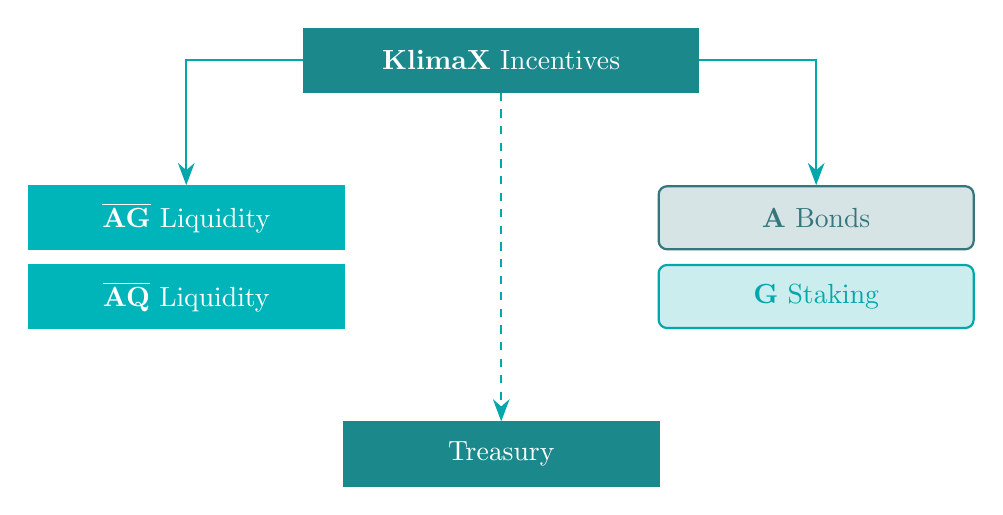
\begin{tikzpicture}[
    title/.style={
        rectangle,
        draw=#1,
        fill=#1,
        thick,
        minimum width=5cm,
        minimum height=0.8cm,
        text=white,
        align=center,
        %rounded corners=3pt
    },
    liquidity/.style={
        rectangle,
        draw=#1,
        fill=#1,
        thick,
        minimum width=4cm,
        minimum height=0.8cm,
        text=white,
        align=center
    },
    token/.style={
        rectangle,
        draw=#1,
        fill=#1!20,
        thick,
        minimum width=4cm,
        minimum height=0.8cm,
        text=#1,
        align=center,
        rounded corners=3pt
    },
    gnode/.style={
        circle,
        draw=peacock_blue,
        fill=white,
        minimum size=1cm,
        inner sep=0pt,
        thick,
        text=gtoken,
        font=\large\bfseries
    },
    arrow/.style={
        -{Stealth[length=8pt]},
        thick,
        #1
    },
    dash_arrow/.style={
        -{Stealth[length=8pt]},
        thick,dashed,
        #1
    }
]

% Title at top
\node[title=teal] (gtitle) at (0,3) {\KG{} Incentives};

% Central G node
%\node[gnode] (gnode) at (0,2) {\G{}};

% Left side - Liquidity pools
\node[liquidity=blue_green] (agliq) at (-4,1) {\AG{} Liquidity};
\node[liquidity=blue_green] (aqliq) at (-4,0) {\AQ{} Liquidity};

% Right side - Bonds and Staking
\node[token=steel_teal] (aBonds) at (4,1) {\A{} Bonds};
\node[token=peacock_blue] (gstaking) at (4,0) {\G{} Staking};

% Bottom - Treasury
\node[liquidity=teal] (treasury) at (0,-2) {Treasury};

% Draw arrows from G node
\draw[arrow=peacock_blue] (gtitle.west) -| (agliq.north);
\draw[arrow=peacock_blue] (gtitle.east) -| (aBonds.north);
\draw[dash_arrow=peacock_blue] (gtitle.south) -- (treasury.north);
%\draw[arrow=peacock_blue] (gnode) -- (gstaking.west);
%\draw[arrow=peacock_blue] (gnode) -- (treasury);

% Connect title to G node
%\draw[arrow=gtoken] (gtitle) -- (gnode);

\end{tikzpicture}
\end{document}
